\documentclass[a4paper, 12pt]{article}
\usepackage[english]{babel}
\usepackage[a4paper,left=2.5cm, right=2.0cm, top=2.5cm, bottom=2.5cm]{geometry}
\usepackage[utf8]{inputenc}
\usepackage{setspace}
\usepackage{url}
\usepackage{hyperref}
\usepackage{longtable}
\usepackage{lscape}
\usepackage[final]{pdfpages}
\usepackage{graphicx}
\usepackage{colortbl}
\usepackage{multirow}
\usepackage{listings}
\begin{document}
%This file will subsume all of the individual chapters of the project report


%\setstretch{1.50}
\pagestyle{empty}

\begin{center} Project Report \end{center}
\hspace{1cm}
\begin{center} Softwareproject: \end{center}
\begin{center}Spoken Dialog Systems for Elevator Control \end{center}
\begin{center} Universität des Saarlandes \end{center}
\begin{center} Department 4.7 Computational Linguistics and Phonetics \end{center}
\begin{center} Computerlinguistik, B.Sc./M.Sc. \end{center}
\begin{center} Summer term 2015 \end{center} 

\hspace{1cm}
\begin{center}Instructors: Ingmar Steiner, Asad Sayeed, Arif Khan \end{center}

\begin{center} Participants: Anne-Julia Hoffmann, Boyuan Deng, Laura Faust \end{center}


\pagestyle{plain}
\setcounter{page}{1}

%please put in the files you wrote in the corresponding order and space by
%using \input{filename} so that we can compile the entire project report as one

\section{Dialogue System}

\subsection{ASR}

\subsubsection{Acoustic model}
Training etc.
\subsection{Reverberation recordings in the elevator}

\begin{figure}[h]
\hspace*{3cm}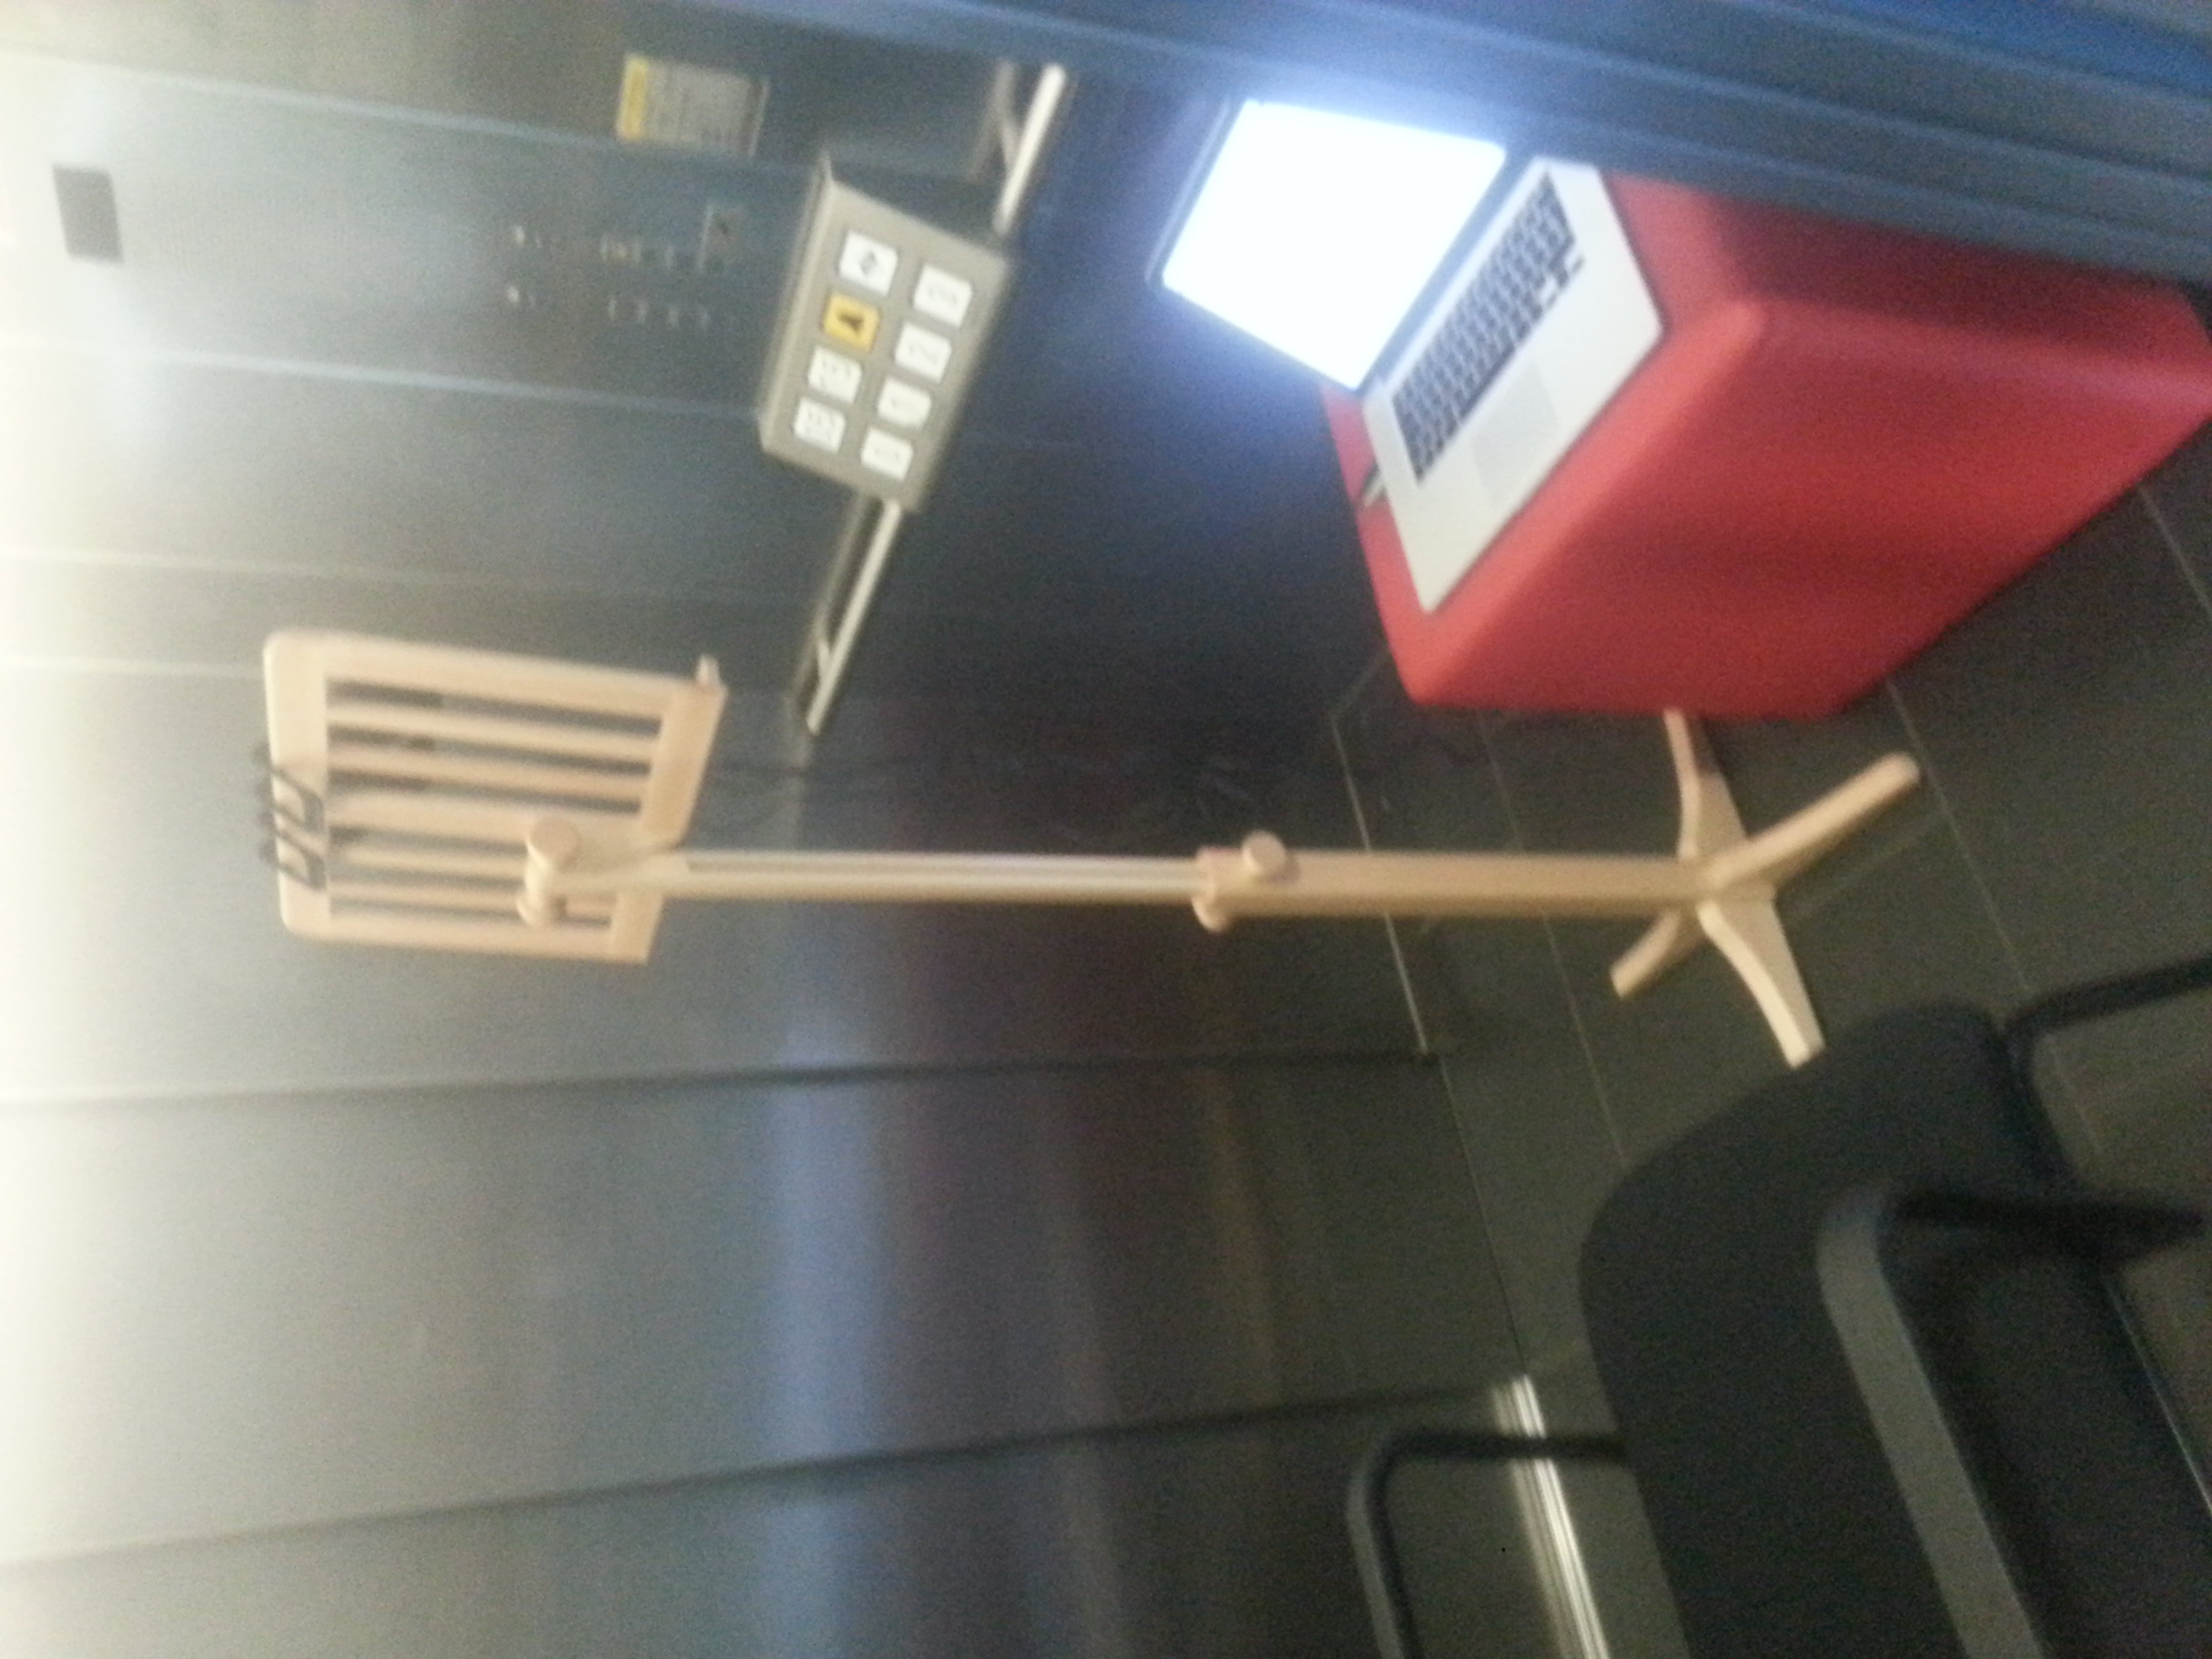
\includegraphics[scale=0.15]{setup_reverberation_rec.jpg}
\caption{Recordings setup.}
\label{fig:recordingsetup}
\end{figure}



\noindent To account for the noise of the elevator, its sound when moving, the sound of the doors opening and closing and the reverberation with open doors on the different floors and other noises from outside of the elevator, recordings were done via the elevator's built-in microphone. 
The setup used for this can be seen in picture \ref{fig:recordingsetup}.
It consisted of two loudspeakers positioned on a music stand at the height of approximately 150cm, at a distance of approximately 20cm from the elevator's microphone. 
The recordings made in the lab were played through the loudspeakers and recorded with Praat via the elevator's microphone. 
While the recordings were being played, the elevator was moved between the floors, its doors were opened and closed and kept with its doors opened and closed on different floors.


\subsubsection{Language model}

%\input{jsgf_summary.tex}

\subsection{Dialog-manager}

The dialog manager is responsible for keeping track of the conversation and deciding the next move of the system for each input. The domain of our project is fairly limited. Most conversational situations consist of the user naming a location and the machine taking the action of moving to that location and reassuring the user that it had understood the command. This can described by deterministic If...then... statements. A dialog manager that models the conversation flow as an deterministic FSA is well-suited for our needs.
When choosing the dialog manager for our project we considered the following factors: It had to be open source, preferably Java, well documented.
We were also looking for code that was actively maintained.
We reviewed a few potential contenders:
\begin{itemize}
\item[IrisTK] \hfill \\
TODO
\item[InproTK] \hfill \\
The most exciting asset of this dialog manager was incremental processing.
The code is well maintained and actively developed. 
However, we failed to build a demo that uses incremental features due to the lack of documentation so we dropped this option.
\item[OpenDial] \hfill \\
OpenDial is probably the most popular open source dialog manager.
After successfully implementing a short domain-relevant demo we opted for this manager.
For more detailed description of OpenDial see next section.

\end{itemize}
\subsubsection{Opendial}
\label{sec:opendial}
\subsection{Dialog Manager - this small chapter has to be synchronized with the previous one - }

After a sound has been recognized as speech and the words have been extracted by the grammar, the system needs to decide which action to take and also perform it.
This process is done in the so called ”Dialog Manager”. When and how the system should react to speech is defined in this program.

For the speaking elevator ”EllaVator” the Dialog Manger ”Open Dial” was used.
Therefore I would like to give a quick introduction to the Dialog System Open Dial in the following Chapter.

\subsection{Open Dial}

Like most Dialogue Managers Open Dial also consist of three different components which interact to create a dialogue. 

The first component is responsible for the recognition of language. 
In Open Dial this component is called „ Natural Language Understanding model”. 
The output of the first process is passed on to the next component which checks if there was a instruction given which action should be  be performed upon that input. 
Such actions might be showing something on a GUI, starting a task or simply selecting an answer to the users input. 
In OpenDial this part is called „Dialog Manager”.
The third and last component is called „Natural Language Generation module” and is basically the opposite of the „Natural Language Understanding model”. 
The „Natural Language Generation model” Generates Language from the output of the „Dialog Manger”. 
Though the component is named ”Natural Language Generation model” the output of a Dialogue System is not necessarily speech, but the output is often designed so that it can be easily used to generate speech with a TTS. 
This is also the case for open Dial. 
Open Dial also offers a GUI where the dialogue (input, as well as output) is displayed without having to use further plug-ins.

\subsubsection{Domain}

All of the components mentioned above are located in the so called Domain file.
A dialogue designer working with Open Dial will in most cases just have to work on this one file. For easier readability, it can of course be split into smaller files, which will then have to be imported into one single file. \newline

In this file the users input will be first transformed into a XML structure and then further processed.
Some systems fill this structure with semantic information. 
OpenDial however basically passes variables through the components of the system. 
The dialogue designer can then assigns values to those variables which will ultimately determine the flow of the dialogue. 
There is a convention for the naming of the variables, they can however be named to the dialogue designers liking. 
As all information is being passed through variables the correct naming is important though. 
All three components have a slot ”trigger” at the very beginning of their structure. 
The value given to this slot has to be the name of all variables which are to activate this component.
For example giving the component this trigger: 
\textless model trigger=”a\_u” \textgreater will make it respond to all variables with the name ”a\_u”.  \newline

So the variables in Open Dial do not only carry the value through the system but their names also determinate which module should continue to process that variable. The most common way to link them was described above: Having the Natural Language Understanding module process the users input, the Dialogue Manager process that input and then responding using the Natural Language Generation module. 
In case there is no further processing needed one might also decide to directly link Natural Language Understanding module to Natural Language Generation module. 
If the System should maybe ask a question after having said something, it might also be possible that the dialogue designer might want to trigger the Natural Language Generation twice, either linking Natural Language Generation to Natural Language Generation module or Natural Language Generation module to the Dialogue Manager which again links back to the Natural Language Generation module. \newline

The domain-file is first subdivided into three parts as they each represent one components these parts are called modules. 
The modules themselves are again subdivided into rules. Every rule in this file represents one command. 

\subsubsection{Natural Language Understanding module}

The first model to receive input is the ”Natural Language Understanding module” (NLU). 
Depending whether further plug-ins are used this module will get its input either directly from the user or from the plug-in.
Open Dials NLU component is able to work with plain text input from the user, but in the case of the Ellavator project the User shall also be able to use speech commands to operate the elevator, therefore the NLU in this project receives input from the grammar file of the Sphinx plug-in.
The grammar of the Sphinx plug-in already does part of the work, which would be usually done by the NLU alone.
There is only a very limited amount of commands which the elevator is able to execute.
Each of those can be however be triggered by various expressions. As different people will use different words and structures to express themselves.
Therefore a domain-file that should be capable of doing something should have at least one rule which can be activated by at least one expression. \newline

In the example shown below there is a rule which models the command of changing a direction.
A rule consists of at least one case-expression.
A case-expression itself consists of a ”condition” and an ”effect”.
 In the ”condition”, as the name already states the Dialogue Designer can define under which circumstances a case-expression will match the users input.
These conditions are connected using a logical operator.
In most cases one would want to use the conditions ”or” as either one of those expressions should trigger the rule.
 The ”effect” will be the value passed on to the TM.
As stated before this is done by assigning a variable of the proper name a value.
In the case of the example below the variable is assigned the value of the function of changing to floor to the level of the given parameter. 
\newline


\textless rule \textgreater \newline
\indent \indent \textless  case \textgreater \newline
\indent \indent \indent \textless condition operator=”or”  \textgreater \newline\indent \indent \indent \indent \textless if var=”u\_u” value=”go to second floor” relation=”contains”/  \textgreater \newline
\indent \indent \indent \indent \textless if var=”u\_u” value=”take me up to the second floor” \newline
\indent \indent \indent \indent relation=”contains”/ \textgreater \newline
\indent  \indent \indent \indent \textless if var=”u\_u” value=”second floor” relation=”contains”/ \textgreater \newline
\indent \indent \indent \textless /condition \textgreater \newline
\indent \indent \indent \textless effect prob=”1” \textgreater \textless set var=”a\_u” value=”Request(second)” / \textgreater \newline
\indent \indent \indent \textless /effect \textgreater \newline
\indent \indent \textless /case \textgreater \newline
\indent \indent \textless case \textgreater \newline
\indent \indent \indent \textless condition operator=”or” \textgreater \newline
\indent \indent \indent \indent \textless if var=”u\_u” value=”go to thrid floor” relation=”contains”/ \textgreater \newline
\indent \indent \indent \indent \textless if var=”u\_u” value=”take me up to the third floor” relation=”contains”/ \textgreater \newline
\indent \indent \indent \indent \textless if var=”u\_u” value=”third floor” relation=”contains”/ \textgreater \newline
 \indent \indent \indent \textless /condition \textgreater \newline
\indent \indent  \textless effect prob=”1” \textgreater \textless set var=”a\_u” value=”Request(third)” / \textgreater \newline
\indent \indent  \textless /effect \textgreater \newline
\indent \indent \textless /case \textgreater \newline
\indent \textless /rule \textgreater \newline


In the example above one rule is shown.
This one rule includes two different commands.
They are gathered in one rule as the both are orders to switch a floor.
The only difference is the floor level they have.
Resulting in different parameters which are given to the function of the variable ”a\_u” in the ”effect” slot. \newline



As stated before every user will use different words to express themselves.
To cover up all possible utterances for a command is impossible.
But one should try to at least cover the most common ones,  to make the dialogue more natural for the user.
This part can also be done in the grammar of Sphinx.
Open Dial offers a few possibilities to do so.
The first possibility would be to simply list all the expressions as it is shown in the figure above.
But as can be easily seen in the example above, there is only a small difference between the sentences.
If one would like to cover all possible sentences by merely enlisting them the Domain file will not only get extremely huge it will also be hard to read.
Therefore it is recommended to use the following expressions which will help to keep the Domain file smaller and easier to read which will make it less prone to mistakes and errors if used in the right amount. \newline


\begin{tabular}{|ll|}
\hline
	a? & The word „a” may or may not occure in the expression .  \\
\hline
	(a \textbar b \textbar... \textbar x) & One of the symboles written	in the brakets has to occure.\\
\hline
	(a \textbar b \textbar... \textbar x))? & One of the symboles written in the brakets may or may not occure.  \\
\hline
\end{tabular}
\newline

This table shows the expressions which can be used to structure a the NLU. \newline \newline

In the example used above all three user-utterances could be shortened down using the expression:
\textless if var=”u\_u” value=”(go \textbar take me) (up to the)?  second floor” relation=”contains”/ \textgreater

Using this expressions is therefore recommended.

\subsubsection{Dialogue Manager}

If the variable which was assigned in the NLU module was named correctly it should, in most cases, first be passed trough the Dialogue Manager (DM).
In the Dialogue Manager the effect of a rule is triggered. A mapping occurs which links the input provided by the NLU to another structure that will trigger a reaction of the system.
As was said in the last subchapter, values in Open Dial are saved within and passed trough variables, the input from the NLU will therefore be assigned to another variable. \newline
Just like all other modules each command in the DM is divided into rules, each of them having a condition, when they are to be activated. 
Therefore in this component the output of the NLU component will be matched against all conditions in the DM. 
As soon as one matching rule is found, that rule is triggered which sends the ”effect” of that rule.
The effect of a rule is saved into a variable.
If no further work, like printing information on a GUI is done, one could argue, that all the DM does is basically linking two variables, the one given in the ”condition” to the variable written in the ”effect”.
Of course not all parameters do have to be listed.
It is sufficient to merely put a placeholder in curly brackets to indicate that there is a parameter to be passed on. \newline


\textless rule id=”Movement” \textgreater \newline
 \indent \indent \textless case \textgreater \newline
\indent \indent \indent \textless condition \textgreater \newline
\indent \indent \indent \indent \textless if var=”a\_u” value=”Request(\{x\})” / \textgreater \newline
 \indent \indent \indent \textless /condition \textgreater \newline
 \indent \indent \indent \textless effect util=”1” \textgreater \newline 
 \indent \indent \indent \indent \textless set var=”a\_m” value=”floor(\{x\})” / \textgreater \newline
 \indent \indent \indent \textless /effect \textgreater \newline
\indent \indent \textless /case \textgreater \newline
\indent \textless /rule \textgreater \newline

The figure above shows  a rule called ”Movement” which links the users input ”Request” with any parameter to the effect of that input.
The variable with the name ”a\_m” and the value ”floor” with the input of the Request is send.
The parameter specified in the placeholder ”x” written in curly brackets.

\subsubsection{Natural Language Generation module}

The last part of the system generates the speech. 
Without any further plug-ins this will be done by printing the text to the GUI.
As stated before, this component basically does the opposite of the Natural Language Understanding module. 
Instead of transforming the users input into an XML structure, the system takes the last components output, which is a variable embedded in an XML structure and transforms it back to plan text, either spoken if plug-ins are used or printed on the GUI, if no plug-ins are used. \newline

Each command is again given its own ”rule” and ”case” structure, in which ”condition and effect are included. 
The effect of this rule is saved in a variable but also used as output for speech. \newline

\textless rule \textgreater \newline
\indent \indent \textless case \textgreater \newline
\indent \indent \indent \textless condition \textgreater \newline 
\indent \indent \indent \indent \textless if var=”a\_m” value=”floor(\{x\})” / \textgreater \newline
\indent \indent \indent \textless /condition \textgreater \newline
\indent \indent \indent \textless effect util=”1” \textgreater \newline 
\indent \indent \indent \indent \textless set var=”u\_m” value=”Okay, I will now take you to the {x} floor.” / \textgreater \newline
\indent \indent \indent \textless /effect \textgreater \newline
\indent \indent\textless /case \textgreater \newline
\indent \textless /rule \textgreater \newline

The example above shows one rule from an NLG module. 
In this rule a variable to which a function  is assigned, triggers the speech output of an acknowledgement from the system.



\subsection{TTS}

\section{Implementation details}
\subsection{Raspberry pi}
\subsubsection{Raspberry Pi Virtualization}
By setting up a virtual Raspberry Pi, we can further test our software without physically accessing the Raspberry Pi and burning disk images all the time, even after all automatic tests are passed.

Raspberry Pi uses an ARM processor, so the only tool available to emulate it on PCs is \texttt{qemu}.

Basically we follow the instructions from \url{http://www.linux-mitterteich.de/fileadmin/datafile/papers/2013/qemu_raspiemu_lug_18_sep_2013.pdf} but use the latest Raspbian image instead, which can be downloaded from \url{https://www.raspberrypi.org/downloads/}.

And download \texttt{kernel-qemu} from \url{http://web.archive.org/web/20150214035104/http://www.xecdesign.com/downloads/linux-qemu/kernel-qemu} because the original page is unavailable.

Currently this solution has several drawbacks, mostly notable ones are low speed and lack of serial port support.

\vspace{\baselineskip}

Note:

\begin{itemize}
\item The second line of \texttt{/etc/udev/rules.d/90-qemu.rules} is indeed \texttt{KERNEL=="sda?", SYMLINK+="mmcblk0p\%n",}, there is a typo in the picture.
\item Although the new RPi 2 model has an ARMv7 processor, Raspbian is still compiled into ARMv6 (for compatibility with old models), so emulating with \texttt{-cpu arm1176} is reasonable.
\end{itemize}
\subsection{Serial control of the elevator}
The Elevator is controlled by sending a hex encoded signal via serial cable.
In order to move the elevator to floor three, we are sending a signal which is interpreted as a move command to floor three.
We can also send a special "heartbeat" signal that will make the elevator respond with the information about the current floor it is on.
So, when the user enters the elevator cabin and asks to take him to certain floor, the user utterance is recognized and the corresponding floor signal is sent.
After the elevator receives the signal it should close the doors and start moving if everything went well.

% we need a few pics here when we finish the setup
%\begin{figure}
%\center{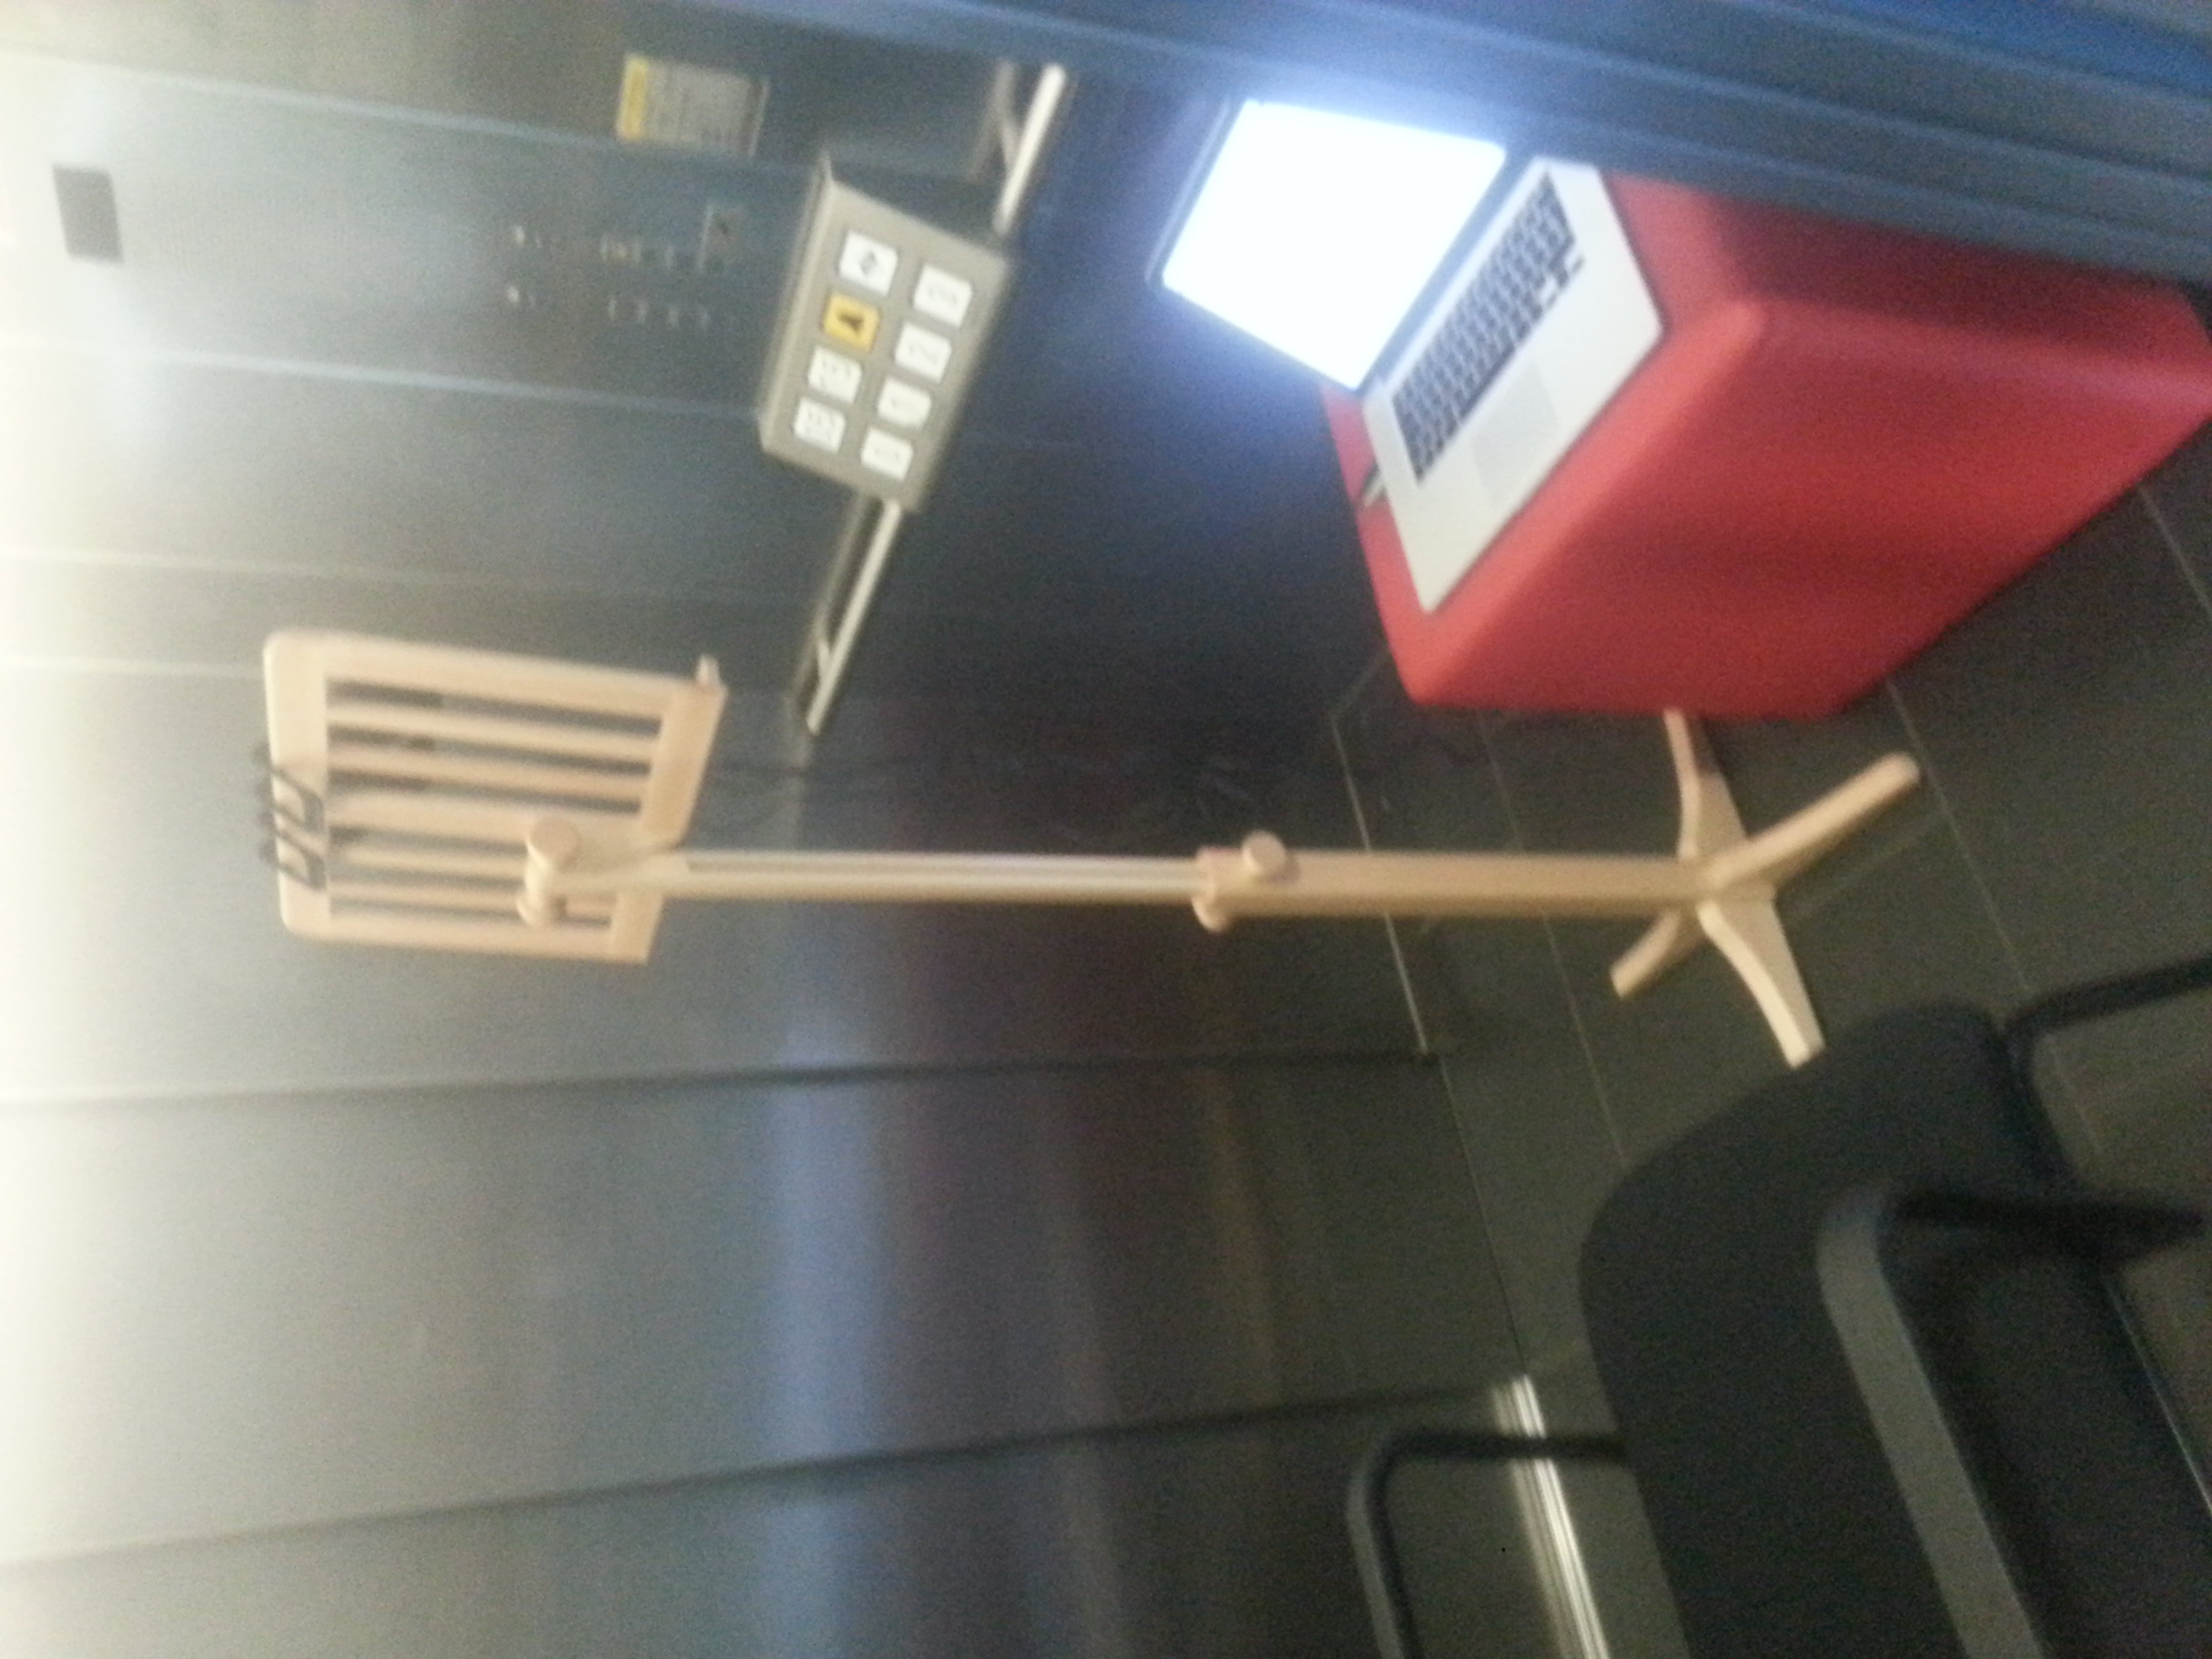
\includegraphics[scale=0.10, angle=-90]{setup_reverberation_rec.jpg}}
%\caption{Recordings setup.}
%\label{fig:recordingsetup}
%\end{figure}

Before working on serial implementation we reviewed several java libraries for serial communication: pi4j, javax.comm, RXTX.
It was decided to stay with RXTX, since pi4j was not stable enough and javax.comm didn't have freely available sources.
Serial implementation follows mainly RXTX examples provided \href{http://rxtx.qbang.org/wiki/index.php/Two_way_communcation_with_the_serial_port}{online} as well as source files of the original project.
For example, floor hex codes and "heartbeat" signal were taken from the original source code.
We also reused several methods from old source files, like the ones that deal with "heartbeat" processing logic.

\subsubsection{Serial cable connection setup}
Raspberri Pi 2 should be connected to the elevator via DE-9 type serial port.
After numerous of unsuccessful attempts to connect Raspi to the serial port via its GPIO pins, we decided to buy a USB to serial converter. 
The new converter worked fine out-of-the-box.
We successfully sent test signals via serial port from Raspi to desktop PC and vice verse.
After running several tests between Raspi and desktop PC we decided to test serial connection to the elevator.

We managed to send a signal to the elevator via serial port however the elevator was able to move only to one specific floor (0.5 which corresponds to 1 floor).
The signal was interpreted by the elevator as a command to move to floor 1.
We suspect that this is due to insufficient power (5V) of Raspi USB to serial connector.
The signal gets garbled upon transmission.
We believe that if we manage to boost the serial port power up to 12V the connection should stabilize and work correctly.

\subsubsection{Serial connection implementation}
Within EllaVator project you can find the following classes that handle serial connection and data transmission between Raspberry Pi and the elevator: \texttt{ElevatorController.java, SerialControllerInterface.java, SerialPortController.java}.\\
\texttt{ElevatorController.java} is basically a wrapper class that instantiates \texttt{SerialPortController} with predefined constant values for serial connection.
These values are important and should not be changed unless you decide to replace Raspberri Pi.\\
Serial port name = \textbf{\texttt{/dev/ttyAMA0}} default serial port on Raspberry Pi.\\
\href{https://en.wikipedia.org/wiki/Serial\_port\#Speed}{Baudrate} = \textbf{38400} proved to work well with our implementation.\\
\href{https://en.wikipedia.org/wiki/Serial\_port\#Data_bits}{Bits} = use \textbf{8} bits.\\
\href{https://en.wikipedia.org/wiki/Serial\_port\#Stop_bits}{Stopbits} = use \textbf{1}.\\
\href{https://en.wikipedia.org/wiki/Serial\_port\#Parity}{Data correction or Parity} = set to \textbf{NO\_PARITY}.\\

All the constants are are kept in \texttt{SerialControllerInterface.java} class.
After we instantiate \texttt{SerialPortController} the following public methods become available through \texttt{ElevatorController} class: \texttt{getCurrentFloor()} and \texttt{pushButton()}. 
Method \texttt{pushButton()} is invoked whenever we want elevator to move to specific floor.
It accepts integers from 0 to 5 where each integer corresponds to specific floor (see \texttt{SerialControllerInterface.java}). 
Method \texttt{getCurrentFloor()} should return the integer which represents current floor the elevator is on.
This method triggers \texttt{getReceivedBytes}, \texttt{findValidSubstrings} (taken from original code) and \texttt{checkMessage} (taken from original code).
Method \texttt{findValidSubstrings} triggers \texttt{addByteStringToArrayList}.
Each method is accompanied by extensive information, please read it first.

\subsection{Serial port testing}
It is technically impossible to test Raspi and elevator connection without opening the elevator control panel.
Therefore, for testing we used an old laptop with serial port and a desktop PC.
For testing purposes we wrote several python scripts, pi4j java testing tool and a small RXTX java implementation.
We also used such shell utilities as minicom.
\\

There were 3 testing phases.

1 testing:

We used python pyserial implementation to test serial connection between Raspi, laptop and PC.
After several unsuccessful attempts to use pi4j and GPIO pins connection, we switched to USB serial converter.
Raspi successfully sent the signals via serial port using USB converter.
We also managed to test the serial connection between a laptop and a desktop PC.
Everything worked as expected.
\\

2 testing:

We connected the laptop to the elevator via laptop serial port with a simple serial cord.
Small RXTX serial port utility was used to send the signals from the laptop.
Everything worked correctly and we managed to control the elevator from the laptop by sending the appropriate signals.
\\

3 testing:

We connected Raspi to the elevator using USB serial converter.
The same RXTX serial port utility was used to send the signals to the elevator.
However whatever floor we tried to send the elevator to it moved to floor 1. 
We suspect that Raspi simply does not have enough power to support serial connection to the elevator.
\\

Our next steps:

Find a way how to boost Raspi serial port power from 5V to 12V.
If it fails, drop Raspi completely and use a variant of desktop PC with an SD drive.

\subsection{Testing}
Software testing is an essential process in modern software development, in particular in the process of quality assurance (QA) of software.
As the name indicates software testing verifies whether the software does what it is supposed to do.
But though invented for this purpose, software testing can accomplish more than that.
Tests also help to maintain the features that have been developed in the past and protects them from being destroyed accidentally by new code.
On top of that tests can help developers to understand or remember what exactly the code does, as tests are generally easier to understand than code.
Tests provide examples of how the existing code is supposed to be used and therefore provide a very useful addition to the documentation.
The most extreme incarnation of testing might be a development process called Test Driven Development.
In this process tests are even written before the actual code.

Generally there at least two types of tests: unit and integration tests.
While unit tests are thought to test small components (e.g. classes) in isolation, integration tests verify how these components work as a whole.

Seeing time constraints and also our lack of experience, we decided not to be as strict with testing, and we put a focus on integration testing.
All tests are placed in the \texttt{test} source set, i.e. under \texttt{src/test}.
There they can be found automatically by gradle when executing \texttt{./gradlew test} in the commandline.
We used TestNG\footnote{http://testng.org/doc/} as our testing framework.

\subsection{Development tools}

\subsubsection{Gradle}
Gradle\footnote{http://gradle.org/} is a build automation tool and simplifies the build process drastically.
Instead of having a readme file that explains how to build the project, building the project is as easy as executing \texttt{./gradlew build} on the command line.

Gradle is configured in the file \texttt{build.gradle}.
Although it looks like a configuration file, it is actually fully functional code written in Groovy\footnote{http://www.groovy-lang.org/}, a programming language based on Java.

We included a Gradle wrapper in the repository.
This file called \texttt{gradlew} (and \texttt{gradle.bat} for windows) download and run the right Gradle version when executed.
It is recommended to use this file instead of using this file instead of any other locally installed Gradle, because it might be another version of Gradle.

The file \texttt{settings.gradle} specifies the gradle project structure by declaring several subprojects.
There is the opendial subproject, which is a copy of the dialog manager OpenDial\footnote{http://www.opendial-toolkit.net/}.
Next we have the pi4j subproject, which is a copy of Pi4j\footnote{http://pi4j.com/}.
We use it for serial port communication.
Next we have the sphinx4 subproject, consisting of sphinx4-core and sphinx4-data, which is a copy of the speech recognition software Sphinx4\footnote{https://github.com/cmusphinx/sphinx4}.
These subprojects are all forked on github from the originals, eventually adapted for our purposes and then included as a Git submodule.
Finally we have a subproject called prompts, that is our own making.
It contains example audio prompts for our application, that are used for the acoustic model training and for testing.

\subsubsection{GitHub}
GitHub is a web platform for collaboration using git, which is a version control system. 
We used this system to allow several people work on the same project at the same time without overwriting each others changes.

For some of our dependencies (Sphinx, pi4j, OpenDial) we used git submodules to include them into our project. 
This gave us the possibility to adapt the original code for our purposes if necessary.
In order to download these dependencies when you clone the repository, you must therefore execute
\begin{lstlisting}[language=bash]
git clone https://github.com/EllaVator/EllaVator.git --recursive
\end{lstlisting}
or init and update all of the subprojects individually.

\subsubsection{Travis}
\subsection{Continuous integration with Travis CI}

Continuous integration is based on the idea that all developers send their changes to a common code repository as soon as possible, as we did on GitHub. 
Additionally these changes should be tested before they are merged into the main code repository. 
In order to do this automatically, it is necessary to automate the build process completely, as we did using Gradle.
If the build succeeds, all unit and integration tests can be executed, which prevents non-working code to enter the main repository if the error is covered by a test case.
This procedure is much better than having each developer running the tests before committing the changes to the main repository for a couple of reasons.
Firstly it does not rely on the developer to run all the tests which can be easily forgotten or skipped because the developer does not see the whole effect his modification has.
Secondly the project is built in a “neutral” environment that should be a close copy of the production environment if possible. 
This way for example code that runs fine on the developer's Windows machine but not on Linux can be detected.

As it integrates seamlessly into GitHub, we decided to use Travis CI as our continuous integration service. Each pull request gets marked by colors: yellow means the build is still running, red means failed build or failed test, green says everything is OK. In each pull request there is a link to Travis that gives details about the build process, too.

Travis is configured by a file named \texttt{.travis.yml} in the root directory of the project. 
It is not even necessary to specify that the build process is handled by Gradle.
Travis can detect this automatically, given that we specify groovy as our project language (\texttt{language: groovy}).
We needed to use Java 8 because this is a minimum requirement for Opendial.
Also, Travis must install the \texttt{sox} command, which is used to extract single sentences from our test audio files in the prompts subproject.
Finally, we cache the gradle files to speed up the build process (otherwise the Gradle wrapper will download Gradle every time).

Each developer can add Travis to his own repositories, too.
That way failures can be detected even before sending a pull request.
Travis can be activated by signing up on \url{https://travis-ci.org/} using your GitHub account.
Then go to your profile page on Travis and activate the GitHub repositories you want to be watched (which must contain a \texttt{.travis.yml} file).
From then on every push to these repositories will trigger Travis to build and run tests and send an email about the result.



\section{Quick installation instructions}
\subsection{Ubuntu}


These installation instructions have been tested on Ubuntu 14.04.

If you have not installed git on your system, you should do this first:
\begin{lstlisting}[language=bash]
sudo apt-get install git
\end{lstlisting}

This program is the version control system we used and helps to keep changes by different developers in sync.
For details see the section on Github.

Now you can download the project files using the \texttt{git clone} command.
Navigate to the folder where you want to place the project files and execute:
\begin{lstlisting}[language=bash]
git clone https://github.com/EllaVator/EllaVator.git --recursive
\end{lstlisting}

This will create a folder named \texttt{EllaVator} inside the current directory and put the downloaded files inside.
Please note that you should use the \texttt{--recursive} flag here in order to download all the nessecary files, including the subprojects.

Now enter the created folder:
\begin{lstlisting}[language=bash]
cd EllaVator
\end{lstlisting}

Our project requires Java 8. If you haven't installed it already, you can do so using the following commands:
\begin{lstlisting}[language=bash]
sudo add-apt-repository ppa:webupd8team/java
sudo apt-get update
sudo apt-get install oracle-java8-installer
\end{lstlisting}

Now you can build or run the project using one of the following commands:
\begin{lstlisting}[language=bash]
./gradlew build
./gradlew run
\end{lstlisting}



\include{bibliography}

\end{document}
